\documentclass[12pt]{article}

% ── Codificación y tipografía ──────────────────────────────────────────────────
\usepackage[utf8]{inputenc}
\usepackage[T1]{fontenc}
\usepackage{lmodern}
\usepackage{amssymb}
\usepackage[spanish,es-tabla]{babel}
\usepackage{microtype}

% ── Geometría ─────────────────────────────────────────────────────────────────
\usepackage[left=3cm, right=2.5cm, top=3cm, bottom=2.5cm]{geometry}
\setlength{\headheight}{24.02pt}
\addtolength{\topmargin}{-12.01pt}

% ── Gráficos y colores ────────────────────────────────────────────────────────
\usepackage{xcolor}
\usepackage{graphicx}
\usepackage{pgfgantt}
\usepackage{tikz}
\usetikzlibrary{shapes.geometric}

% ── Tablas ────────────────────────────────────────────────────────────────────
\usepackage{booktabs}
\usepackage{array}
\usepackage{multirow}
\usepackage{tabularx}
\usepackage{longtable}
\usepackage{colortbl}
\usepackage{makecell}

% ── Formato y estructura ──────────────────────────────────────────────────────
\usepackage{fancyhdr}
\usepackage{titlesec}
\usepackage{parskip}
\usepackage{enumitem}
\usepackage{hyperref}
\usepackage{amssymb}
\usepackage[htt]{hyphenat}
\usepackage{float}

% ── Paleta de colores ─────────────────────────────────────────────────────────
\definecolor{azulppal}{RGB}{0,70,127}
\definecolor{azulclaro}{RGB}{173,216,230}
\definecolor{grisoscuro}{RGB}{64,64,64}
\definecolor{grisclaro}{RGB}{245,245,245}
\definecolor{naranja}{RGB}{204,85,0}
\definecolor{verdeok}{RGB}{34,139,34}
\definecolor{g1}{RGB}{41,128,185}
\definecolor{g2}{RGB}{39,174,96}
\definecolor{g3}{RGB}{211,84,0}
\definecolor{g4}{RGB}{142,68,173}
\definecolor{g5}{RGB}{192,57,43}
\definecolor{tabhead}{RGB}{0,70,127}
\definecolor{tabrow}{RGB}{235,243,252}

% ── hyperref ──────────────────────────────────────────────────────────────────
\hypersetup{
  colorlinks=true, linkcolor=azulppal, urlcolor=azulppal, citecolor=azulppal,
  pdftitle={Informe Académico -- Capstone Analytics},
  pdfauthor={Sebastián Ramírez, Vicente Ramírez, Joaquín Parraud}
}

% ── Encabezado y pie ──────────────────────────────────────────────────────────
\pagestyle{fancy}
\fancyhf{}
\fancyhead[L]{\small\color{azulppal}\textbf{Informe Académico -- Simulación Panadería de Supermercado}}
\fancyhead[R]{\small\color{grisoscuro}Abril--Mayo 2026}
\fancyfoot[C]{\small\thepage}
\renewcommand{\headrulewidth}{0.5pt}
\renewcommand{\headrule}{\hbox to\headwidth{\color{azulppal}\leaders\hrule height 0.5pt\hfill}}

% ── Secciones ─────────────────────────────────────────────────────────────────
\titleformat{\section}{\large\bfseries\color{azulppal}}{\thesection.}{0.5em}{}[\titlerule]
\titleformat{\subsection}{\normalsize\bfseries\color{grisoscuro}}{\thesubsection.}{0.5em}{}
\titleformat{\subsubsection}{\normalsize\itshape\color{grisoscuro}}{\thesubsubsection.}{0.5em}{}
\setlist[itemize]{topsep=2pt,itemsep=1pt,leftmargin=*}
\setlist[enumerate]{topsep=2pt,itemsep=1pt,leftmargin=*}
% Limits ToC to Section and Subsection only
\setcounter{tocdepth}{2} 



% ─────────────────────────────────────────────────────────────────────────────
\begin{document}
% Force A4 portrait for all pages (pdflatex defaults to letter without a4paper).
\pdfpagewidth=210mm
\pdfpageheight=297mm
\setlength{\parskip}{6pt}

% ══════════════════════════════════════════════════════════════════════════════
%  PORTADA
% ══════════════════════════════════════════════════════════════════════════════
\begin{titlepage}
\centering
\vspace*{0.4cm}

\includegraphics[width=0.36\linewidth]{../UDD.png}\\[0.9cm]
{\color{azulppal}\rule{\linewidth}{2.5pt}}\\[0.5em]
{\Huge\bfseries\color{azulppal} Informe Académico}\\[0.4em]
{\large\bfseries\color{grisoscuro} Proyecto Capstone Analytics}\\[0.2em]
{\color{azulppal}\rule{\linewidth}{1pt}}\\[0.8em]
{\Large\itshape\color{grisoscuro}
  Simulación de Eventos Discretos:\\[0.3em]
  Proceso de Fabricación de Pan\\
  en Panadería de Supermercado}

\vspace{0.85cm}
\begin{tabular}{@{}ll@{}}
  \textbf{Universidad:}      & Universidad del Desarrollo \\[3pt]
  \textbf{Ramo:}             & Capstone Analytics \\[3pt]
  \textbf{Código:}           & IIC511AD \\[3pt]
  \textbf{Profesor:}         & Victor Vera, PhD \\[3pt]
  \textbf{Documento:}        & Proyecto de Simulación -- Informe Académico \\[3pt]
  \textbf{Fecha:}            & 19 de mayo de 2026 \\[3pt]
\end{tabular}

\vfill
\begin{flushright}
{\small\color{grisoscuro}
\textbf{Integrantes}\\[4pt]
Joaquín Parraud\\
Sebastián Ramírez\\
Vicente Ramírez}
\end{flushright}
\vspace{0.4cm}
{\color{azulppal}\rule{\linewidth}{2.5pt}}\\[0.3em]
{\small\color{grisoscuro} Capstone Analytics IIC511AD -- Ingeniería Civil Industrial -- Universidad del Desarrollo}
\end{titlepage}

\tableofcontents

% ══════════════════════════════════════════════════════════════════════════════
\newpage
\section{Introducción}
% ══════════════════════════════════════════════════════════════════════════════

Este Informe Académico documenta el proceso de desarrollo del modelo de simulación de eventos discretos construido para la panadería de un supermercado. A diferencia del Informe Técnico --orientado a la decisión gerencial--, este documento relata las decisiones de modelamiento adoptadas, su justificación, las dificultades encontradas y la metodología empleada en cada etapa.

El sistema bajo estudio es una panadería que produce diez variedades de pan fresco para abastecer la sala de ventas de autoservicio del supermercado entre las 09:00 y las 21:00 horas. El problema declarado por la jefatura es un nivel inaceptable de quiebres de stock que genera pérdidas de venta directas. La hipótesis operacional es que el problema no radica en el volumen de demanda --conocido y cuantificado-- sino en la combinación y coordinación de recursos: número de panaderos, manipuladores, hornos, máquinas, horario de inicio y política de secuenciamiento de producción.

\medskip
\noindent\colorbox{grisclaro}{%
\parbox{\dimexpr\linewidth-2\fboxsep\relax}{%
\vspace{2pt}
\textit{¿Cuál es la combinación mínima de recursos ---panaderos, manipuladores, hornos, mezcladoras, amasadoras y horario de operación--- junto con la política de secuenciamiento de producción, que garantiza un nivel de servicio de al menos 95\% de demanda satisfecha en todos los tipos de pan?}
\vspace{2pt}
}}

% ══════════════════════════════════════════════════════════════════════════════
\newpage
\section{Definición del problema y alcance}
\label{sec:definicion}
% ══════════════════════════════════════════════════════════════════════════════

\subsection{Definición cuantitativa del problema}

La panadería de un supermercado enfrenta un nivel de servicio global de \textbf{68,3\%} en su configuración base (2~panaderos, 1~manipulador, 1~horno, inicio a las 06:00). Esto implica que aproximadamente 1 de cada 3~kg de pan demandados no está disponible en el momento en que el cliente lo requiere. Los productos críticos son Marraqueta (22,7\% de satisfacción), Hallulla Integral (39,0\%) y Marraqueta Integral (58,4\%), que concentran el 56\% de la demanda diaria total (8.200~kg/día).

El problema declarado por la jefatura es la frecuencia e intensidad de los quiebres de stock durante el horario de atención al público (09:00--21:00), que generan pérdidas de venta directas y degradan la experiencia de compra. La hipótesis operacional es que el origen no está en el nivel de demanda ---conocido y cuantificado--- sino en la combinación de recursos (panaderos, manipuladores, hornos) y en la política de secuenciamiento de producción.

\subsection{Alcance del modelo}

\textbf{Incluido en el modelo:}
\begin{itemize}
  \item Producción de 10~variedades de pan fresco con sus tiempos de proceso, familias de horneado y perfiles de demanda horaria.
  \item Recursos: panaderos, manipuladores, hornos batch industriales, mezcladoras y amasadoras.
  \item Demanda estocástica: llegadas de clientes con perfil horario variable, elección probabilística de productos y cantidad de compra triangular por tipo.
  \item Inventario en sala y registro de quiebres de stock a nivel de evento.
  \item Política de secuenciamiento de producción: modos push y pull con variantes.
\end{itemize}

\textbf{Excluido del modelo:}
\begin{itemize}
  \item Logística de abastecimiento de materias primas (se asume disponibilidad continua).
  \item Costos económicos de producción, energía o personal (el KPI es servicio, no costo).
  \item Variabilidad en los tiempos de proceso (los tiempos de proceso son deterministas, calibrados desde los datos entregados).
  \item Canales de venta fuera de la sala de autoservicio (despacho a domicilio, otros formatos).
\end{itemize}

\subsection{Criterio de éxito}

El estudio busca identificar la \textbf{combinación mínima de recursos} que garantice un nivel de servicio de \textbf{al menos 95\%} de demanda satisfecha \textbf{simultáneamente} en todos los tipos de pan. El criterio es simultáneo: un escenario que logre 99\% global pero tenga un producto al 60\% se considera insatisfactorio.

% ══════════════════════════════════════════════════════════════════════════════
\newpage
\section{Sistema bajo estudio}
% ══════════════════════════════════════════════════════════════════════════════

\subsection{Descripción del proceso productivo}

La panadería opera en un ciclo diario en el que debe abastecer la sala de ventas entre las 09:00 y las 21:00 horas. La producción comienza antes de la apertura para garantizar disponibilidad inicial de todas las variedades. El proceso productivo de cada variedad incluye, en secuencia: pesado y dosificación de ingredientes, mezclado (intervención manual del panadero más ciclo automático de mezcladora), amasado manual, reposo o fermentación en masa, dividido y formado, fermentación final, horneado batch, enfriamiento y reposición a sala.

\subsection{Hornos y familias de horneado}

Los hornos son de tipo industrial (piso o rotativo) y operan en modo batch por corrida: se cargan, hornean y descargan completamente antes de iniciar la siguiente corrida. Los diez tipos de pan se agrupan en tres familias de horneado según tiempo de cocción ---14, 18 y 21 minutos---, y no se permite mezclar familias en una misma carga. La capacidad máxima por corrida es de 6~carros con 18~bandejas cada uno (108~bandejas en total). La carga mínima para disparar una corrida es 600~kg (50\% de la capacidad), con un tiempo máximo de espera de 15~minutos. El cambio entre corridas de la misma familia no requiere setup; el cambio entre familias requiere 5~minutos.

\subsection{Demanda y composición de compra}

La demanda diaria total alcanza 8.200~kg distribuidos entre los diez tipos de pan, con un perfil horario conocido. Cada cliente que llega compra uno, dos o tres tipos de pan con probabilidades 50\%, 35\% y 15\% respectivamente. La cantidad comprada por tipo sigue una distribución triangular (mínimo, moda, máximo) específica para cada producto.

% ══════════════════════════════════════════════════════════════════════════════
\newpage
\section{Modelo conceptual}
% ══════════════════════════════════════════════════════════════════════════════

\subsection{Entidades y recursos}

El modelo distingue dos tipos de entidades en flujo: \textbf{clientes} que llegan a la sala de ventas según un perfil horario y consumen inventario, y \textbf{lotes de producción} que recorren la ruta productiva desde el pesado hasta la reposición. La separación entre cliente y lote es una decisión deliberada que evita acoplar la lógica de consumo con la lógica de producción.

Los recursos del modelo son: panaderos (que ejecutan las etapas manuales del proceso productivo), manipuladores (responsables de carga y descarga del horno, traslados internos y reposición a sala), hornos batch industriales, mezcladoras, amasadoras y los elementos físicos de transporte interno (carros y bandejas).

\subsection{Inventario y eventos}

El inventario en sala se representa mediante un vector de stock por tipo de pan, no como entidades físicas. Esta decisión simplifica el modelo computacionalmente sin perder precisión en los KPIs relevantes (nivel de servicio, quiebres, demanda perdida). Los eventos críticos del sistema son: llegada de cliente, consumo de inventario, generación de lote, disparo de corrida de horno, reposición a sala y cierre de turno.

\subsection{Variables de decisión}

Las variables de decisión del estudio son:
\begin{itemize}
  \item Número de panaderos, manipuladores, hornos, mezcladoras y amasadoras.
  \item Hora de inicio de operación productiva (antes de la apertura de la sala).
  \item Política de secuenciamiento de producción: prioridad al producto con menor stock, prioridad al producto con mayor demanda esperada, secuencia fija por familias, o estrategia híbrida.
\end{itemize}

\subsection{KPI principal}

El criterio cuantitativo de éxito es el porcentaje de demanda satisfecha por tipo de pan, que debe ser igual o superior al 95\% para todos los productos. Como criterio secundario para discriminar entre configuraciones que cumplen el estándar, se utiliza la utilización de recursos (minimización del costo operativo).

% ══════════════════════════════════════════════════════════════════════════════
\newpage
\section{Decisiones de modelamiento}
% ══════════════════════════════════════════════════════════════════════════════

Las decisiones que se describen a continuación quedaron cerradas antes de comenzar la construcción del modelo, con el fin de evitar que distintos integrantes implementaran lógicas inconsistentes en paralelo.

\subsection{Clave única por producto}

Cada tipo de pan se identifica internamente por un índice numérico (\texttt{ProductoIdx}) y no por su nombre. Esta clave se propaga por todas las tablas, states y processes del modelo. La motivación es robustez: el lookup por nombre es frágil cuando se importan archivos Excel con espacios extra, acentos inconsistentes o correcciones tipográficas.

\subsection{Demanda como cliente individual}

La demanda se modela como llegadas de clientes individuales según una tabla de tasas horarias (\texttt{Rate\_ClientesHora}), calibrada desde el perfil de demanda en kg/hora dividido por el consumo esperado por cliente. Esta representación se prefirió sobre una demanda agregada por pulsos horarios porque permite capturar la variabilidad en la composición de compra (1, 2 o 3 tipos por cliente) y registrar quiebres a nivel evento.

\subsection{Inventario como state vectorial}

El stock en sala se representa con un state vectorial de 10 posiciones (\texttt{StockSala[i]}), una por tipo de pan, y no como entidades físicas circulando en el modelo. Esta decisión reduce drásticamente la carga computacional y mantiene la trazabilidad sobre los KPIs.

\subsection{Hornos: tres colas lógicas por familia}

El horno batch se implementa con tres colas lógicas, una por familia de horneado. Cada lote ingresa con su requerimiento de carros y bandejas, y la lógica de formación de carga selecciona lotes de una misma familia mientras la suma de carros no exceda la capacidad. La política de setup se evalúa mediante un proceso explícito que consulta una matriz de cambios entre familias.

\begin{figure}[H]
\centering
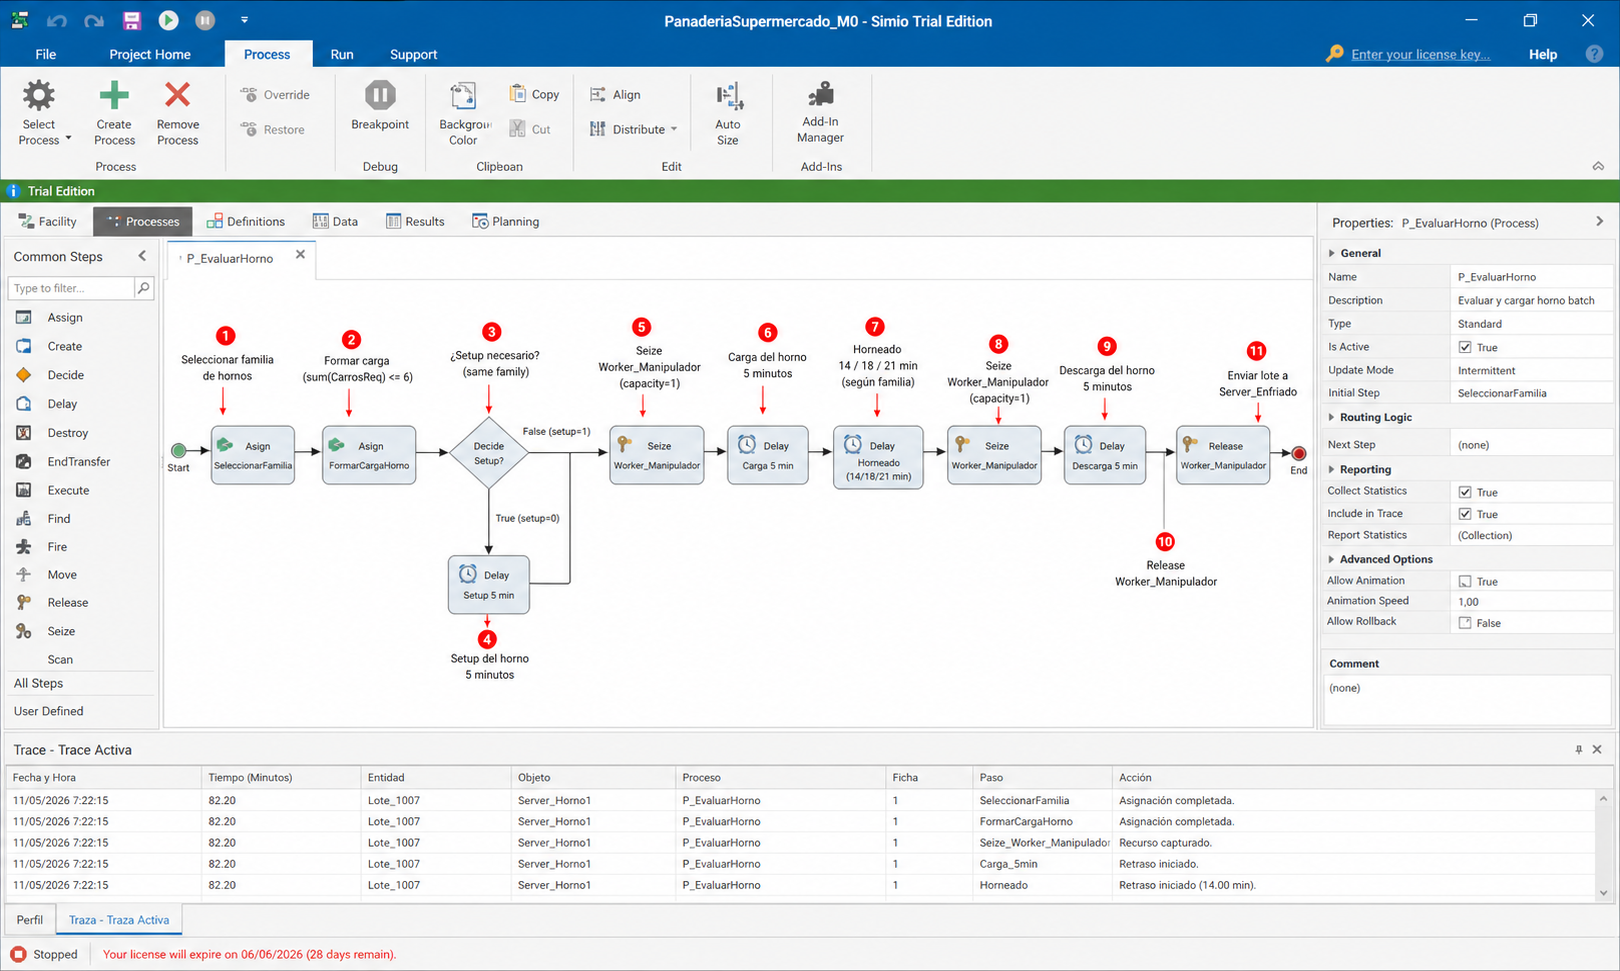
\includegraphics[width=0.85\linewidth]{../GuiaImplementacionSimio/figures_ai/ai_06_oven_batch_process.png}
\caption{Esquema conceptual del horno batch: tres colas lógicas por familia, formación de carga por carros y bandejas, y política de setup entre familias.}
\label{fig:horno-acad}
\end{figure}

\subsection{Recursos humanos}

Los manipuladores se modelan como \texttt{Worker} de Simio con schedules de turno explícitos, lo que permite capturar caminata, colaciones (45~min) y descansos (2$\times$15~min). Los panaderos se modelan como \texttt{Secondary Resource} lógico (capacidad sin caminata física), una simplificación deliberada porque el desplazamiento físico del panadero no es relevante para los KPIs del estudio.

\subsection{Ruta productiva única}

A pesar de que los diez tipos de pan tienen tiempos distintos en cada etapa, todos siguen la misma secuencia física de etapas. Por lo tanto el modelo usa una ruta única con tiempos parametrizados desde la tabla de etapas por producto, en lugar de rutas separadas o \texttt{Sequence Tables}.

\begin{figure}[H]
\centering
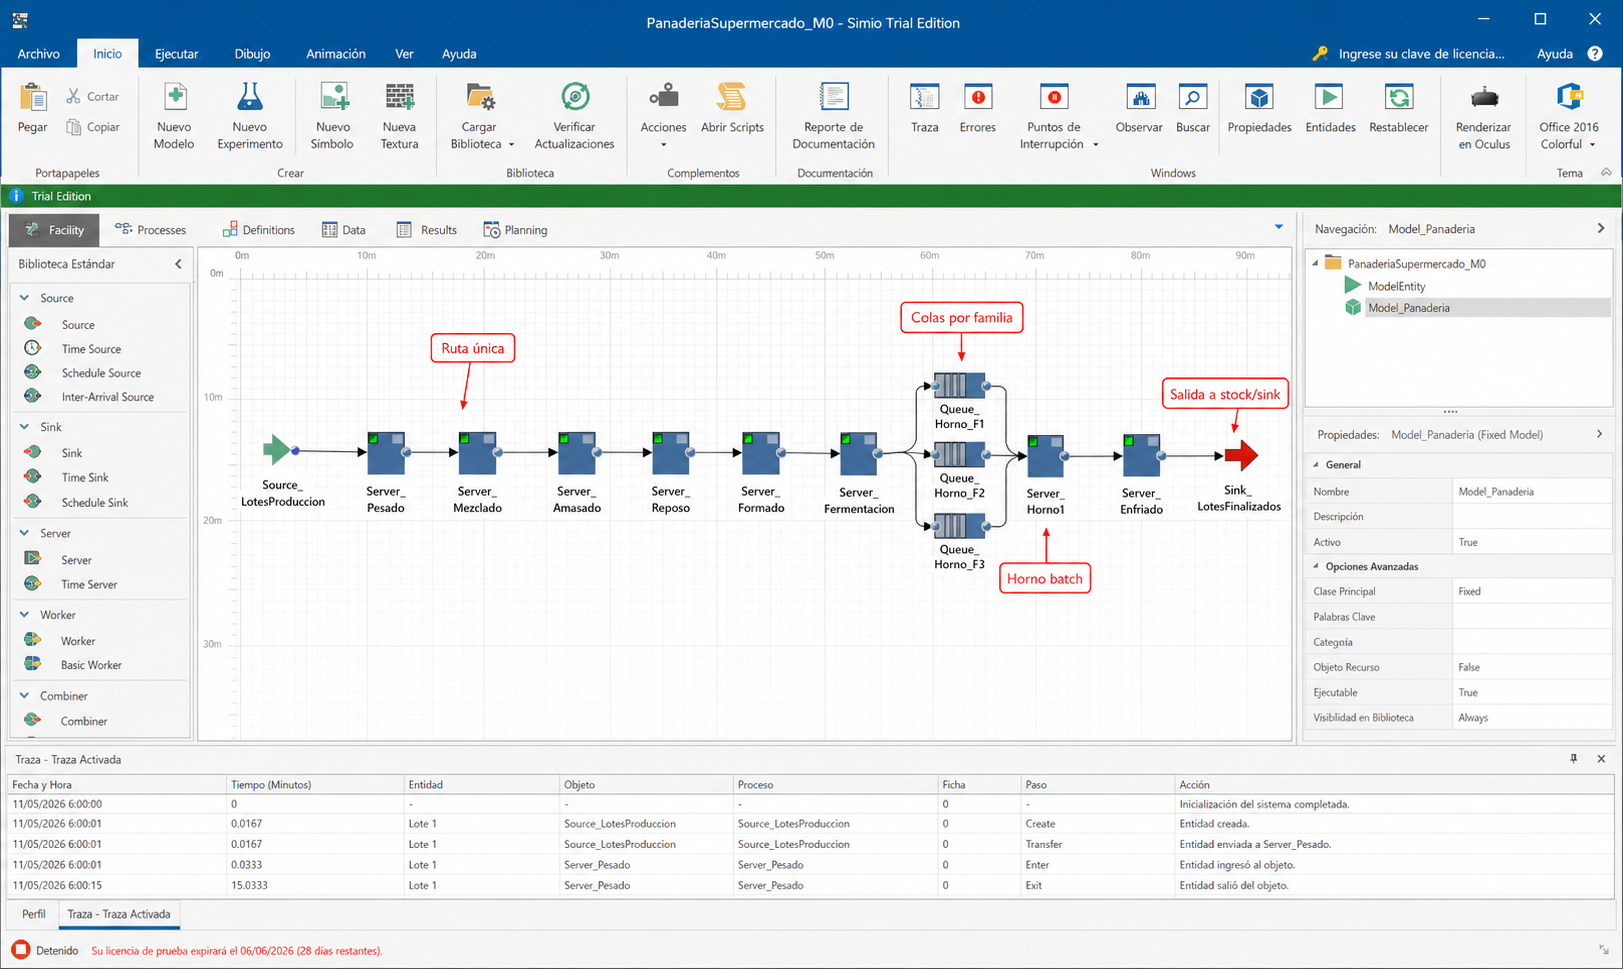
\includegraphics[width=0.85\linewidth]{../GuiaImplementacionSimio/figures_ai/ai_05_production_route.png}
\caption{Ruta productiva única recorrida por todos los tipos de pan, con tiempos parametrizados por producto desde la tabla de etapas.}
\label{fig:ruta-acad}
\end{figure}

% ══════════════════════════════════════════════════════════════════════════════
\newpage
\section{Implementación en Simio}
% ══════════════════════════════════════════════════════════════════════════════

La construcción del modelo siguió una secuencia modular incremental de siete etapas (M0 a M7), con verificación obligatoria al cierre de cada módulo antes de comenzar el siguiente.

\begin{table}[H]
\centering
\caption{Secuencia modular de implementación}
\label{tab:modulos}
\renewcommand{\arraystretch}{1.3}
\begin{tabularx}{\textwidth}{lX}
\toprule
\rowcolor{tabhead}\color{white}\textbf{Módulo} & \color{white}\textbf{Contenido} \\
\midrule
M0 & Creación de Data Tables, states, properties, processes mínimos y \texttt{Source\_InitModel} \\
\rowcolor{tabrow}
M1 & \texttt{Source\_Clientes}, demanda con \texttt{Rate\_ClientesHora}, inventario por \texttt{Assign}; calibración con stock infinito \\
M2 & Servers de producción, flujo dummy, ruta única, registro de WIP y ciclo \\
\rowcolor{tabrow}
M3 & Horno: M3A funcional de a un lote, luego M3B batch completo por familia y carros \\
M4 & Workers, schedules, secondary resources \\
\rowcolor{tabrow}
M5 & Consolidación de KPIs, verificación por checklist, validación de baseline \\
M6 & Experimentos: Controls, Responses y matriz de escenarios \\
\rowcolor{tabrow}
M7 & Documentación final y reproducibilidad \\
\bottomrule
\end{tabularx}
\end{table}

\subsection{Diccionario de tablas}

El modelo se alimenta de un conjunto cerrado de tablas con nombres canónicos: \texttt{Tbl\_ProductoIndice}, \texttt{Tbl\_EtapasProducto}, \texttt{Tbl\_DemandaHoraLong}, \texttt{Tbl\_ProbEleccionHoraLong}, \texttt{Tbl\_MixCompraCliente}, \texttt{Tbl\_StockPolitica}, \texttt{Tbl\_HornoFamilia}, \texttt{Tbl\_SetupHorno}, \texttt{Tbl\_RecursosInstancia}, \texttt{Tbl\_Escenarios} y \texttt{Tbl\_Supuestos}. Adicionalmente se crea \texttt{Rate\_ClientesHora} como \texttt{Rate Table} (no como Data Table normal) para alimentar la tasa de llegadas variable.

\subsection{Processes principales}

La lógica del modelo se concentra en procesos con triggers explícitos. Entre los más relevantes:

\begin{itemize}
  \item \texttt{P\_InitModel}: inicialización del stock y de los states de escenario al inicio de la corrida.
  \item \texttt{P\_GenerarDemandaCliente}: sortea número de productos a comprar y dispara la cadena de elección y consumo.
  \item \texttt{P\_ElegirProductos}: muestreo sin reemplazo con probabilidades normalizadas por hora.
  \item \texttt{P\_ConsumirInventario}: descuenta stock, acumula demanda satisfecha y registra quiebres.
  \item \texttt{P\_EvaluarHorno}, \texttt{P\_FormarCargaHorno}, \texttt{P\_AplicarSetupHorno}: lógica del horno batch.
  \item \texttt{P\_ReponerSala}: traslado de pan fresco desde el área de enfriamiento al inventario de sala.
\end{itemize}

% ══════════════════════════════════════════════════════════════════════════════
\newpage
\section{Datos de entrada y tratamiento}
% ══════════════════════════════════════════════════════════════════════════════

\subsection{Archivos fuente}

Los datos del caso provienen de tres archivos entregados por la cátedra: \texttt{parametros\_proceso\_panaderia.xlsx} (parámetros del proceso productivo y de hornos), \texttt{perfil\_demanda\_por\_hora\_panaderia.xlsx} (demanda en kg por hora y tipo) y \texttt{probabilidades\_eleccion\_por\_hora.xlsx} (probabilidad horaria de elección de cada tipo).

\subsection{Capa ETL previa}

Antes de importar a Simio, los archivos pasan por una capa de transformación que: (a) verifica consistencia interna y unidades; (b) convierte los datos a formato \texttt{long} normalizado por \texttt{ProductoIdx}; (c) calcula la tasa de llegadas de clientes a partir del perfil de kg/hora y el consumo esperado por cliente; (d) construye la tabla maestra de productos con sus distribuciones triangulares de compra.

\subsection{Análisis cuantitativo de los datos de entrada}

\textbf{Concentración de la demanda:} la distribución de los 8.200~kg/día no es uniforme. Los cuatro productos de mayor demanda ---Marraqueta (2.000~kg, 24,4\%), Hallulla (1.700~kg, 20,7\%), Pan Hot Dog (1.200~kg, 14,6\%) y Marraqueta Integral (800~kg, 9,8\%)--- concentran el 69,5\% de la demanda total. Los seis restantes suman el 30,5\%, con Bocado de Dama como el menos demandado (220~kg, 2,7\%). Esta concentración implica que los recursos productivos estarán mayoritariamente orientados hacia los productos de Familia~2 (18~min de horneado), que reúnen el 58,5\% de la demanda.

\textbf{Perfil horario y horas pico:} el perfil de demanda horaria registra los picos de consumo entre las 12:00--14:00 y las 18:00--20:00, coincidiendo con horarios de almuerzo y merienda. En las horas pico la tasa de llegadas de clientes puede ser hasta 3$\times$ la tasa del horario valle. Esto implica que el modelo debe capturar la variabilidad temporal de la demanda y no puede asumir una llegada uniforme.

\textbf{Caracterización por familia de horneado:}
\begin{itemize}
  \item Familia~1 (14~min): Pan Hot Dog, Dobladita, Bocado de Dama $\Rightarrow$ 1.770~kg/día (21,6\%)
  \item Familia~2 (18~min): Marraqueta, Hallulla, Hallulla Integral, Amasado $\Rightarrow$ 4.880~kg/día (59,5\%)
  \item Familia~3 (21~min): Marraqueta Integral, Ciabatta, Baguette $\Rightarrow$ 1.550~kg/día (18,9\%)
\end{itemize}

La concentración en Familia~2 genera presión diferenciada sobre el horno en franjas de alta demanda, lo que justifica el diseño de la política híbrida de secuenciamiento.

\subsection{Registro de supuestos}

Toda decisión que no proviene directamente de los archivos fuente queda registrada en la tabla \texttt{Tbl\_Supuestos}, junto con su valor base, fuente, sensibilidad esperada y estado. Esto incluye los tiempos de etapas no especificados, los tiempos de desplazamiento internos y la política de corridas por debajo de la carga mínima.

% ══════════════════════════════════════════════════════════════════════════════
\newpage
\section{Verificación y validación}
% ══════════════════════════════════════════════════════════════════════════════

\subsection{Verificación}

La verificación responde a la pregunta: ¿el modelo fue construido correctamente? Su protocolo se basa en una lista de chequeo aplicada en M5:
\begin{itemize}
  \item Los lotes siguen la secuencia correcta de etapas para cada variedad.
  \item Los panaderos se capturan y liberan en los momentos correctos.
  \item El horno rechaza cargas mixtas entre familias.
  \item La carga del horno no excede 6~carros ni 108~bandejas.
  \item Los descansos del personal son escalonados y nunca simultáneos para una misma función.
  \item No existen entidades bloqueadas ni colas con crecimiento ilimitado.
\end{itemize}

\subsection{Validación}

La validación responde a la pregunta: ¿el modelo representa de manera aceptable el sistema? En contexto académico se apoya en: (a) coherencia del orden de magnitud de los resultados con el análisis de capacidad estático; (b) análisis de sensibilidad de primer nivel (duplicar la capacidad del horno debe mejorar los quiebres); (c) revisión cruzada por integrantes que no construyeron el módulo revisado.

Una prueba específica de calibración consiste en correr el modelo con inventario inicial infinito y sin producción activa: la demanda diaria generada debe converger a los 8.200~kg/día esperados dentro de un margen de $\pm$5\% en 30~réplicas.

% ══════════════════════════════════════════════════════════════════════════════
\newpage
\section{Diseño experimental}
% ══════════════════════════════════════════════════════════════════════════════

\subsection{Factores y niveles: plan original}

La matriz experimental contemplaba los siguientes factores de decisión:

\begin{itemize}
  \item Número de panaderos: 2, 3, 4.
  \item Número de manipuladores: 1, 2, 3.
  \item Número de hornos: 1, 2, 3.
  \item Número de mezcladoras y amasadoras (rango por definir según análisis preliminar).
  \item Hora de inicio de operación: 04:00, 05:00, 06:00.
  \item Política de secuenciamiento: cuatro opciones (menor stock, mayor demanda esperada, secuencia fija por familias, híbrida).
\end{itemize}

\subsection{Escenarios efectivamente ejecutados}

Por restricciones de tiempo, se ejecutaron cinco escenarios con énfasis en variación de recursos humanos, número de hornos y política de lotes. La hora de inicio (06:00 en todos los casos) y el número de mezcladoras y amasadoras (1~de cada una) se mantuvieron fijos. Los escenarios elegidos corresponden a las variaciones de mayor interés gerencial: el efecto de un panadero adicional, el efecto de un segundo horno, el efecto de compartir estaciones y un caso de referencia teórica para conocer el techo del sistema.

La descripción detallada de cada escenario se presenta en la Tabla~\ref{tab:escenarios-acad} de la Sección~\ref{sec:resultados}.

\subsection{Protocolo de réplicas: limitación}

El protocolo diseñado contemplaba 20--30~réplicas por escenario. Por restricción de tiempo, se ejecutó 1~réplica por escenario. Los resultados son indicativos pero no tienen validez estadística formal: no es posible calcular intervalos de confianza ni realizar pruebas de comparación entre escenarios con una sola réplica. Esta es la limitación metodológica más importante del estudio y debe considerarse al interpretar las diferencias entre casos.

El horizonte de simulación es un día operacional completo: desde la hora de inicio productivo (06:00 en todos los casos ejecutados) hasta las 21:00 horas.

\subsection{Análisis de sensibilidad}

Sobre la configuración recomendada se planearon perturbaciones para verificar robustez: demanda total $\pm$20\%, cambio en el mix hacia variedades de horneado largo, tiempos de fermentación aumentados en 15\%, y variación en la política de setup del horno. Este análisis formal no fue ejecutado. La comparación entre los cinco escenarios ejecutados permite extraer sensibilidades indirectas, que se detallan en la Sección~\ref{sec:sensibilidad}.

% ══════════════════════════════════════════════════════════════════════════════
\newpage
\section{Supuestos de modelación}
\label{sec:supuestos}
% ══════════════════════════════════════════════════════════════════════════════

\subsection{Simplificaciones adoptadas}

El modelo incorpora supuestos en dos categorías: aquellos derivados de los datos entregados por la cátedra, y aquellos adoptados por ausencia de información empírica.

\textbf{Supuestos con base en datos entregados:}
\begin{itemize}
  \item El perfil de demanda horaria (kg/hora por tipo de pan) se toma directamente de \texttt{perfil\_demanda\_por\_hora\_panaderia.xlsx}.
  \item Los tiempos de etapas productivas y temperaturas de horneado provienen de \texttt{parametros\_proceso\_panaderia.xlsx}.
  \item Las probabilidades de elección de producto por franja horaria provienen de \texttt{probabilidades\_eleccion\_por\_hora.xlsx}.
\end{itemize}

\textbf{Supuestos sin respaldo empírico (fuente: criterio del equipo):}
\begin{itemize}
  \item Cantidad comprada por cliente por tipo de pan: distribución triangular con mínimo 0,25~kg, moda 0,75~kg, máximo 2,0~kg. No se disponía de datos de ticket POS ni transaccionales. Sensibilidad estimada: media.
  \item Mezcla de compra: un cliente elige 1 tipo de pan con probabilidad 50\%, 2 tipos con 35\%, 3 tipos con 15\%. Supuesto de comportamiento sin validación transaccional. Sensibilidad: media.
  \item Velocidad de desplazamiento del panadero: 1,2~m/s. Velocidad del manipulador con carro: 0,8~m/s. Impacto bajo sobre los KPIs dado que los tiempos de desplazamiento son pequeños frente a los tiempos de proceso.
  \item Carga mínima del horno: 600~kg. Este valor fue entregado en el enunciado pero es inconsistente con la capacidad por carro (que en kg depende del tipo de pan y no de un umbral global). Se registra como supuesto de alta sensibilidad.
\end{itemize}

\subsection{Justificación y efectos de los supuestos}

El supuesto de mayor impacto potencial es la carga mínima del horno. En la configuración base, esta restricción hace que los lotes de productos de baja demanda deban esperar hasta alcanzar 600~kg o agotar el tiempo de espera de 15~minutos antes de disparar una corrida. Esto reduce la frecuencia de horneado efectiva para productos de Familia~3 (Ciabatta, Baguette, Marraqueta Integral) y explica en parte por qué esos productos tienen niveles de servicio inferiores a pesar de su baja demanda relativa.

La distribución triangular de cantidad comprada por cliente es el segundo supuesto de mayor incertidumbre. Un comportamiento de compra real más concentrado (compras más pequeñas y frecuentes) reduciría los quiebres momentáneos; uno más disperso los agravaría. La ausencia de datos POS es una limitación reconocida del estudio.

% ══════════════════════════════════════════════════════════════════════════════
\newpage
\section{Resultados del modelo}
\label{sec:resultados}
% ══════════════════════════════════════════════════════════════════════════════

\subsection{Escenarios ejecutados}

Se ejecutaron cinco escenarios de simulación con 1~réplica cada uno. La replicación estadística completa (20--30~réplicas) fue planeada pero no completada por restricción de tiempo. Los resultados deben interpretarse como indicativos del comportamiento del sistema, no como estimaciones puntuales con precisión estadística garantizada.

\textbf{Nota sobre nomenclatura:} El archivo de resultados denominado \texttt{Caso A.csv} registra internamente la etiqueta «Caso~K», lo que indica una discrepancia entre el nombre del experimento en Simio y el nombre del archivo exportado. Se asume la correspondencia con el Caso~A descrito en el protocolo experimental.

\begin{table}[H]
\centering
\caption{Definición de los escenarios ejecutados}
\label{tab:escenarios-acad}
\renewcommand{\arraystretch}{1.3}
\begin{tabularx}{\textwidth}{lXcccl}
\toprule
\rowcolor{tabhead}
\color{white}\textbf{Caso} &
\color{white}\textbf{Descripción} &
\color{white}\textbf{Pan.} &
\color{white}\textbf{Man.} &
\color{white}\textbf{Hornos} &
\color{white}\textbf{Inicio} \\
\midrule
\rowcolor{tabrow} Caso~0 & Base: configuración actual; política híbrida & 2 & 1 & 1 & 06:00 \\
Caso~A & +1~panadero; máx.~2 op. en estación de formado & 3 & 1 & 1 & 06:00 \\
\rowcolor{tabrow} Caso~B & Caso~A $+$ 2.°~horno & 3 & 1 & 2 & 06:00 \\
Caso~C & Caso~B $+$ panaderos comparten estaciones & 3 & 1 & 2 & 06:00 \\
\rowcolor{tabrow} Caso~D & Caso~A $+$ lotes de 600~kg forzados (techo teórico) & 3 & 1 & 1 & 06:00 \\
\bottomrule
\end{tabularx}
\end{table}

\subsection{Niveles de servicio por producto}

\begin{table}[H]
\centering
\caption{Porcentaje de demanda satisfecha por producto y escenario}
\label{tab:resultados-nds-acad}
\renewcommand{\arraystretch}{1.3}
\begin{tabularx}{\textwidth}{Xccccc}
\toprule
\rowcolor{tabhead}
\color{white}\textbf{Producto} &
\color{white}\textbf{Caso~0} &
\color{white}\textbf{Caso~A} &
\color{white}\textbf{Caso~B} &
\color{white}\textbf{Caso~C} &
\color{white}\textbf{Caso~D} \\
\midrule
\rowcolor{tabrow} Marraqueta           & 22,73\% & 69,69\% & 69,68\% & 69,69\% & 100,00\% \\
Hallulla                               & 87,56\% & 67,25\% & 67,25\% & 67,24\% & 100,00\% \\
\rowcolor{tabrow} Pan Hot Dog          & 94,70\% & 93,13\% & 63,94\% & 63,94\% & 99,89\% \\
Marraqueta Integral                    & 58,41\% & 100,00\% & 93,91\% & 93,91\% & 100,00\% \\
\rowcolor{tabrow} Hallulla Integral    & 38,95\% & 100,00\% & 97,45\% & 97,85\% & 100,00\% \\
Ciabatta                               & 100,00\% & 97,66\% & 95,64\% & 96,28\% & 97,66\% \\
\rowcolor{tabrow} Baguette             & 95,93\% & 93,91\% & 91,73\% & 92,44\% & 93,91\% \\
Dobladita                              & 90,48\% & 92,20\% & 89,19\% & 89,64\% & 92,20\% \\
\rowcolor{tabrow} Bocado de Dama       & 99,30\% & 89,21\% & 83,73\% & 84,66\% & 89,21\% \\
Amasado                                & 100,00\% & 94,50\% & 90,91\% & 90,91\% & 94,50\% \\
\midrule
\rowcolor{tabrow}\textbf{Total ponderado} & \textbf{68,32\%} & \textbf{84,67\%} & \textbf{79,12\%} & \textbf{79,28\%} & \textbf{98,62\%} \\
\bottomrule
\end{tabularx}
\end{table}

\subsection{Demanda perdida y lotes de producción}

\begin{table}[H]
\centering
\caption{Demanda perdida y producción por escenario}
\label{tab:dem-perdida-acad}
\renewcommand{\arraystretch}{1.3}
\begin{tabularx}{\textwidth}{Xccccc}
\toprule
\rowcolor{tabhead}
\color{white}\textbf{Métrica} &
\color{white}\textbf{Caso~0} &
\color{white}\textbf{Caso~A} &
\color{white}\textbf{Caso~B} &
\color{white}\textbf{Caso~C} &
\color{white}\textbf{Caso~D} \\
\midrule
\rowcolor{tabrow} Demanda total (kg)         & 8.123,7 & 8.110,3 & 8.110,3 & 8.110,3 & 8.110,3 \\
Demanda satisfecha (kg)                      & 5.549,8 & 6.866,6 & 6.417,0 & 6.430,2 & 7.998,1 \\
\rowcolor{tabrow} Demanda perdida (kg)       & 2.574,0 & 1.243,7 & 1.693,3 & 1.680,1 & 112,2 \\
Stockouts (eventos)                          & 2.568 & 1.251 & 1.697 & 1.681 & 110 \\
\rowcolor{tabrow} Lotes liberados (total)    & 31 & 36 & 33 & 35 & 35 \\
Lotes push                                   & 28 & 34 & 29 & 31 & 35 \\
\rowcolor{tabrow} Lotes pull                 & 3 & 2 & 4 & 4 & 0 \\
Setups de horno                              & 32 & 32 & 28 & 30 & 30 \\
\rowcolor{tabrow} Tiempo setup total (min)   & 80 & 80 & 70 & 75 & 75 \\
\bottomrule
\end{tabularx}
\end{table}

% ══════════════════════════════════════════════════════════════════════════════
\newpage
\section{Análisis y discusión}
\label{sec:analisis}
% ══════════════════════════════════════════════════════════════════════════════

\subsection{Diagnóstico del escenario base}

El Caso~0 opera al 68,3\% de nivel de servicio global, con 2.574~kg no vendidos y 2.568 eventos de quiebre en un único día simulado. La Marraqueta --- el producto de mayor demanda (2.000~kg/día, 24,4\% del total) --- solo alcanza un 22,7\% de satisfacción: en la práctica, la sala de ventas queda sin Marraqueta la mayor parte del día. Hallulla Integral (39,0\%) y Marraqueta Integral (58,4\%) también están críticos. Este resultado confirma con evidencia cuantitativa lo que la jefatura observaba cualitativamente.

\subsection{Cuello de botella 1: el panadero como recurso escaso}

Pasar de Caso~0 a Caso~A (agregar 1~panadero, de 2 a 3) eleva el nivel global de 68,3\% a 84,7\%, una mejora de 16,4~puntos porcentuales. Más revelador aún: Marraqueta Integral salta de 58,4\% a 100\% y Hallulla Integral de 39,0\% a 100\%. Esto indica que el 3.er~panadero libera suficiente capacidad productiva para satisfacer completamente la demanda de los dos productos integrales, cuya demanda combinada es de 1.600~kg/día (19,5\% del total).

El panadero es el recurso que controla la tasa de inicio de nuevos lotes (es el recurso primario en las etapas de pesado, amasado y formado). Con 2~panaderos, el sistema debe serializar estos trabajos, creando una cola de espera que retrasa todos los ciclos de producción. El panadero adicional reduce este cuello de manera directa.

\subsection{Cuello de botella 2: el efecto paradójico del segundo horno}

La comparación entre Caso~A y Caso~B es el hallazgo más contraintuitivo del estudio. Agregar un segundo horno (manteniendo los mismos 3~panaderos y 1~manipulador) \emph{reduce} el nivel de servicio global de 84,7\% a 79,1\%: una caída de 5,6~puntos porcentuales. El deterioro más dramático ocurre en Pan Hot Dog, que colapsa de 93,1\% a 63,9\% (pérdida de 386,7~kg/día).

La explicación es sistémica: con 2~hornos, el sistema tiene capacidad de horneado para procesar más corridas simultáneamente. Sin embargo, los panaderos ---que preparan los lotes antes del horneado--- no se duplican. Los 3~panaderos ahora deben alimentar 2~colas de horno simultáneamente, aumentando la competencia por su tiempo entre todos los productos. La política de prioridades de la cola determina qué productos reciben atención primero; Pan Hot Dog aparentemente pierde prioridad, acumulando retrasos que no tenía cuando había un solo horno.

Este resultado ilustra un principio fundamental en sistemas de manufactura: ampliar la capacidad de un recurso no cuello de botella sin escalar el recurso cuello de botella puede degradar el desempeño global.

\subsection{Cuello de botella 3: ciclos de producción insuficientes para productos de baja demanda}

Cuatro productos mantienen niveles inferiores al 95\% incluso en el Caso~D (escenario utópico con lotes de 600~kg forzados): Baguette (93,9\%), Dobladita (92,2\%), Bocado de Dama (89,2\%) y Amasado (94,5\%). Ciabatta se ubica sobre el umbral en este escenario (97,7\%) y no integra este grupo crítico.

La identidad de resultados entre Caso~A y Caso~D para estos cinco productos es significativa: el tamaño de lote no cambia su desempeño. El factor limitante es el número de ciclos de producción completables en el horizonte operativo. Para Baguette, el ciclo completo desde el pesado hasta la reposición a sala dura aproximadamente 133~minutos. Con producción desde las 06:00 hasta las 21:00 y contención de recursos compartidos, solo se logran 3~ciclos al día. Iniciar 2~horas antes añadiría un ciclo completo adicional, lo que proyecta una mejora significativa para este grupo de productos.

\subsection{Impacto de la política de secuenciamiento}

El Caso~D fuerza lotes de exactamente 600~kg, convirtiendo la política en puramente push (0~lotes pull). Este cambio eleva la Marraqueta de 69,7\% a 100\% y la Hallulla de 67,2\% a 100\%. Los lotes push frecuentes de alta cantidad permiten que la sala de ventas mantenga stock continuo de los productos de alta demanda. La política pull del Caso~A (34~push, 2~pull de 36~lotes totales) no alcanza a reponer estos productos a la velocidad a que se consumen.

% ══════════════════════════════════════════════════════════════════════════════
\newpage
\section{Análisis de sensibilidad}
\label{sec:sensibilidad}
% ══════════════════════════════════════════════════════════════════════════════

El análisis de sensibilidad formal (perturbaciones de demanda $\pm$20\%, fermentación $+15\%$, mix hacia Familia~3) no fue ejecutado. Se extrae sensibilidad indirecta de la comparación entre escenarios:

\subsection{Sensibilidad a la política de lotes}

La transición de Caso~A a Caso~D representa, en términos del parámetro de carga mínima del horno, un descenso de 600~kg a 0~kg (lotes forzados). El impacto es $+13,9$~pp en nivel global (84,7\% $\to$ 98,6\%) y una reducción de la demanda perdida de 1.243,7~kg a 112,2~kg ($-91\%$). Esta es la variable de mayor apalancamiento identificada en el estudio.

Sin embargo, la política de lotes de 600~kg forzados no es operacionalmente viable tal como se define en el experimento (implica iniciar corridas con cualquier cantidad disponible, ignorando la restricción de carga mínima del horno). En la práctica, la mejora correspondiente requiere reformular la política de lotes para ser más agresiva en disparar corridas, aceptar corridas parciales con mayor frecuencia, o adelantar el inicio de producción para acumular lotes antes de la apertura.

\subsection{Sensibilidad al número de hornos}

La sensibilidad del sistema al número de hornos es negativa cuando los recursos humanos no se escalan proporcionalmente. Caso~B (2~hornos) tiene peor desempeño que Caso~A (1~horno) en 5,6~pp. El sistema es \emph{robusto a la reducción} de hornos siempre que se mantengan los recursos humanos adecuados, pero \emph{frágil a la adición} de hornos si los panaderos y manipuladores no aumentan en proporción.

\subsection{Sensibilidad a la exclusividad de estaciones}

Caso~C permite a los panaderos compartir estaciones con otro operario presente. El efecto es prácticamente nulo ($+0,2$~pp respecto a Caso~B). El sistema es insensible a esta variable: el problema no es la exclusividad de acceso a las estaciones sino el tiempo de proceso acumulado en cada etapa.

\subsection{Limitación del análisis}

Con 1~réplica por escenario, los resultados no tienen intervalos de confianza calculados. No es posible distinguir estadísticamente si, por ejemplo, la diferencia entre Caso~B (79,1\%) y Caso~C (79,3\%) es significativa o ruido de la simulación. Un análisis robusto requeriría 20--30~réplicas para calcular intervalos de confianza y aplicar pruebas de comparación entre escenarios.

% ══════════════════════════════════════════════════════════════════════════════
\newpage
\section{Reflexión sobre el proceso}
\label{sec:reflexion}
% ══════════════════════════════════════════════════════════════════════════════

\subsection{Decisiones clave}

\textbf{Inventario como state vectorial}: la decisión de representar el stock en sala como un vector de 10~posiciones (\texttt{StockSala[i]}) en lugar de entidades físicas fue fundamental para la viabilidad computacional del modelo. Esta abstracción reduce drásticamente la carga de simulación sin perder precisión en los KPIs relevantes.

\textbf{Lotes y clientes como entidades independientes}: la separación explícita entre el flujo de clientes (que consumen inventario) y el flujo de lotes de producción (que reponen inventario) permitió que los dos subsistemas evolucionaran con lógicas independientes, facilitando la verificación y depuración por etapas.

\textbf{Enfoque modular M0--M7}: la secuencia de módulos con verificación obligatoria al cierre de cada uno fue determinante para controlar la complejidad en un equipo de tres personas trabajando en paralelo sobre el mismo archivo de modelo.

\subsection{Dificultades encontradas}

La etapa más compleja fue la implementación del horno batch (M3). El modelo correcto (M3B: batch completo por familia con formación dinámica de carga) requirió una primera iteración simplificada (M3A: un lote a la vez sin restricción de familia) para verificar la lógica básica antes de introducir las restricciones de capacidad. Sin este paso intermedio, los errores de lógica en la formación de carga habrían sido difíciles de diagnosticar.

La calibración de la tasa de llegadas de clientes (\texttt{Rate\_ClientesHora}) a partir del perfil de demanda en kg/hora requirió un cálculo previo no trivial: convertir kg/hora por tipo de pan a una tasa de clientes/hora requiere asumir el consumo esperado por cliente, que a su vez depende de la distribución de mezcla de compra y las distribuciones triangulares por producto. Este paso fue iterado hasta que la demanda diaria generada en una corrida de calibración (inventario infinito, sin producción) convergió a los 8.200~kg/día dentro de $\pm$5\%.

\subsection{Limitaciones reconocidas}

La limitación más importante del estudio es la ausencia de replicación estadística. Con 1~réplica por escenario, los resultados son indicativos pero no permiten cuantificar la variabilidad del sistema ni construir intervalos de confianza. Esto impide, por ejemplo, determinar si la diferencia entre Caso~B y Caso~C es estadísticamente significativa o si está dentro del ruido de la simulación.

Una segunda limitación es la no ejecución de escenarios con inicio de producción antes de las 06:00. La hipótesis de que un inicio a las 04:00--05:00 resolvería los productos de ciclo largo (Baguette, Dobladita, Bocado de Dama) es plausible pero no está respaldada por un experimento ejecutado.

Finalmente, la inconsistencia de nomenclatura detectada (Caso~A archivado como «Caso~K» en Simio) subraya la importancia de establecer convenciones de gobernanza de datos antes de comenzar el diseño experimental, especialmente cuando se trabaja en equipo con archivos compartidos.

\subsection{Reflexión por integrante}

\textbf{Joaquín Parraud} (construcción del modelo físico en Simio): El aprendizaje principal fue que la arquitectura del modelo --- cómo se conectan objetos, tablas y procesos --- determina la facilidad de extensión posterior. Haber definido el esquema de tablas completo en M0 facilitó enormemente el trabajo de los módulos siguientes. Si tuviese que volver a empezar, dedicaría más tiempo a la especificación del modelo conceptual antes de entrar a Simio.

\textbf{Sebastián Ramírez} (flujo lógico, reglas de producción y verificación): La verificación por checklist en M5 demostró ser más valiosa de lo esperado: identificó tres inconsistencias en la lógica del horno que habrían contaminado todos los experimentos posteriores. La lección es que la verificación formal no es un formalismo académico sino una inversión que paga dividendos al llegar a los experimentos.

\textbf{Vicente Ramírez} (análisis de datos y diseño experimental): El hallazgo más valioso del análisis fue descubrir que Caso~B es peor que Caso~A: sin el modelo de simulación, la decisión natural de la gerencia sería agregar un horno creyendo que aumenta la capacidad. La simulación revela que ese razonamiento falla cuando el cuello de botella está en otro recurso. Ese es el tipo de conocimiento que justifica el uso de simulación sobre el análisis estático.

% ══════════════════════════════════════════════════════════════════════════════
\newpage
\section{Conclusiones}
\label{sec:conclusiones}
% ══════════════════════════════════════════════════════════════════════════════

\subsection{Aprendizajes del estudio}

El estudio confirmó la hipótesis inicial: el sistema bajo su configuración base es estructuralmente incapaz de alcanzar el 95\% de nivel de servicio para todos los tipos de pan. La brecha no se debe al volumen de demanda ---que es técnicamente alcanzable--- sino a la combinación subóptima de recursos y a la ausencia de ciclos de producción suficientes para los productos de menor demanda y ciclo largo.

El hallazgo más significativo es que la adición de capacidad en un recurso que no es el cuello de botella (el horno) puede degradar el desempeño del sistema. Este resultado, contraintuitivo desde la perspectiva del análisis de capacidad estático, solo es visible a través de la simulación dinámica del sistema completo.

La distancia entre el Caso~A (mejor configuración realista, 84,7\%) y el Caso~D (techo teórico, 98,6\%) indica que existe un potencial de mejora de $\sim$14~pp en nivel de servicio sin cambio de dotación de panaderos o número de hornos, solo ajustando la política de lotes. Traducir este potencial a la práctica requiere explorar con mayor detalle la política de disparo de corridas.

\subsection{Comentarios sobre la metodología de desarrollo}

El enfoque modular (M0--M7) con verificación obligatoria por módulo fue la decisión metodológica correcta para un sistema de esta complejidad. Permite detectar errores en la etapa en que se introducen, en lugar de descubrirlos al ejecutar los experimentos cuando el diagnóstico es mucho más costoso.

La separación entre verificación (¿el modelo fue construido correctamente?) y validación (¿el modelo representa el sistema real?) es conceptualmente clara pero operativamente desafiante cuando no se dispone de datos históricos del sistema para comparar. En este caso, la validación se apoyó en coherencia lógica y análisis de órdenes de magnitud, que son métodos válidos en ausencia de datos históricos pero menos concluyentes que una validación empírica.

\subsection{Valor del uso de simulación}

La simulación de eventos discretos aportó tres tipos de conocimiento que un análisis de capacidad estático no puede entregar:

\begin{enumerate}
  \item \textbf{Efectos de interacción no lineales}: el comportamiento del sistema cuando se agrega un segundo horno no puede predecirse con análisis estático porque depende de la dinámica temporal de contención de panaderos entre colas de producción.
  \item \textbf{Cuantificación de la variabilidad}: aunque la replicación fue limitada, el modelo permite en principio cuantificar la variabilidad de los KPIs a través de réplicas, información imposible de obtener con modelos deterministas.
  \item \textbf{Trazabilidad por producto y por hora}: el modelo registra quiebres a nivel de evento (producto, momento, cantidad no atendida), lo que permite identificar no solo cuánto falta sino cuándo y qué producto falla primero, información valiosa para el diseño operacional.
\end{enumerate}

El caso de la panadería es representativo de una clase amplia de sistemas productivos con demanda estocástica, recursos compartidos y restricciones batch donde la simulación es la herramienta analítica apropiada. La metodología desarrollada es transferible a otros contextos del mismo supermercado (carnicería, pescadería, rotisería) con adaptaciones menores al modelo base.

% ══════════════════════════════════════════════════════════════════════════════
\appendix
\newpage
\section{Parámetros del sistema}
% ══════════════════════════════════════════════════════════════════════════════

\subsection{Demanda diaria por tipo de pan}

\begin{table}[H]
\centering
\caption{Demanda diaria esperada y distribución de compra por cliente}
\label{tab:demanda-acad}
\renewcommand{\arraystretch}{1.3}
\begin{tabularx}{\textwidth}{Xccccc}
\toprule
\rowcolor{tabhead}
\color{white}\textbf{\makecell[c]{Tipo de\\pan}} &
\color{white}\textbf{Familia} &
\color{white}\textbf{\makecell[c]{Dem. diaria\\(kg)}} &
\color{white}\textbf{\makecell[c]{Mín. compra\\(kg)}} &
\color{white}\textbf{\makecell[c]{Moda\\(kg)}} &
\color{white}\textbf{\makecell[c]{Máx. compra\\(kg)}} \\
\midrule
\rowcolor{tabrow} Marraqueta           & 2 (18~min) & 2.000 & 0,3 & 1,0 & 2,0 \\
Hallulla                              & 2 (18~min) & 1.700 & 0,3 & 1,0 & 2,0 \\
\rowcolor{tabrow} Pan Hot Dog          & 1 (14~min) & 1.200 & 0,3 & 1,0 & 3,0 \\
Marraqueta Integral                   & 3 (21~min) &   800 & 0,3 & 0,5 & 2,0 \\
\rowcolor{tabrow} Hallulla Integral    & 2 (18~min) &   800 & 0,3 & 0,7 & 1,5 \\
Amasado                               & 2 (18~min) &   380 & 0,3 & 0,8 & 2,0 \\
\rowcolor{tabrow} Ciabatta             & 3 (21~min) &   400 & 0,3 & 0,5 & 1,5 \\
Baguette                              & 3 (21~min) &   350 & 0,3 & 0,5 & 1,0 \\
\rowcolor{tabrow} Dobladita            & 1 (14~min) &   350 & 0,3 & 0,5 & 1,5 \\
Bocado de Dama                        & 1 (14~min) &   220 & 0,3 & 0,5 & 1,0 \\
\midrule
\rowcolor{tabrow}\multicolumn{2}{l}{\textbf{Total}} & \textbf{8.200} & & & \\
\bottomrule
\end{tabularx}
\end{table}

\subsection{Familias de horneado y parámetros del horno}

\begin{table}[H]
\centering
\caption{Familias de horneado y restricciones del horno}
\label{tab:horno-acad}
\renewcommand{\arraystretch}{1.3}
\begin{tabularx}{\textwidth}{lXc}
\toprule
\rowcolor{tabhead}
\color{white}\textbf{Parámetro} & \color{white}\textbf{Descripción} & \color{white}\textbf{Valor} \\
\midrule
\rowcolor{tabrow} Familia~1 (corto)  & Pan Hot Dog, Dobladita, Bocado de Dama & 14~min \\
Familia~2 (medio)                   & Marraqueta, Hallulla, Hallulla Integral, Amasado & 18~min \\
\rowcolor{tabrow} Familia~3 (largo)  & Marraqueta Integral, Ciabatta, Baguette & 21~min \\
Capacidad máxima                    & Carros por corrida & 6~carros \\
\rowcolor{tabrow} Capacidad por carro & Bandejas por carro & 18~bandejas \\
Carga mínima                        & 50\% de capacidad & 600~kg \\
\rowcolor{tabrow} Espera máxima      & Tiempo máximo antes de disparar corrida & 15~min \\
Setup misma familia                 & Cambio de corrida misma familia & 0~min \\
\rowcolor{tabrow} Setup distinta familia & Cambio de familia & 5~min \\
Carga del horno                     & Manipulador requerido, duración & 5~min \\
\rowcolor{tabrow} Descarga del horno  & Manipulador requerido, duración & 5~min \\
\bottomrule
\end{tabularx}
\end{table}

\subsection{Composición de compra por cliente}

\begin{table}[H]
\centering
\caption{Proporción de tipos de pan por visita}
\label{tab:mix-acad}
\renewcommand{\arraystretch}{1.3}
\begin{tabular}{lc}
\toprule
\rowcolor{tabhead}
\color{white}\textbf{Tipos de pan en una visita} & \color{white}\textbf{Probabilidad} \\
\midrule
\rowcolor{tabrow} 1 tipo de pan & 50\% \\
2 tipos de pan (distintos) & 35\% \\
\rowcolor{tabrow} 3 tipos de pan (distintos) & 15\% \\
\bottomrule
\end{tabular}
\end{table}

\end{document}